\documentclass[a4paper]{article}
\usepackage{graphicx}
\usepackage{url}
\usepackage{geometry}
\usepackage{float}
\usepackage{color}
\usepackage{amsmath}
\geometry{
	a4paper,
	total={170mm,257mm},
	left=20mm,
	top=20mm,
}

%opening
\title{Active Matter Seminar Notes}
\author{Ana Bensabat}

\begin{document}

\maketitle

\section{Soft Matter, Active Matter and Active Particles}

\subsection{What is Soft Condensed Matter Physics?}

soft matter is a subfield of condensed matter physics that focuses on systems that are easily deformable under mechanica stress.

In soft condensed matter physics there are well defined or recognizeble structural units, small particles, colloids or long chains of molecules called polymers that consist of many atoms but with interactions weak enough that their collective response is soft and often not captured by linearized or traditional theoreals.

In these types of systems, thermal fluctuations play an important role on the scale of these structural units. The interactions are usually on the order of $k_B T$. 

Unlike the usual cases in hard condensed matter physics, the systems are easily perturbed and the response is often non linear. They are also, often out of equilibrium and flow easily. They exhibit a disorded structured, unlike the usual crystals we are used to seeing in solid state physics.

\subsection{What is active matter?}

Active matter is matter that is able to harvest and harness energy from the environment in a way that gives rise to complex collective behaviours and forms of self-organisation.

It is a very general concept or term that applies to systems in several different scales and scientific domains, from physics and chemistry to biology and societal systems. These types of self-organisation occur at different time and length scales, \textit{in a way that almost resembles the universility that we see in phase transitions?}.

Phenomena such as flocking and schooling arise when self-propulsive, out-of-equilibrium actors interact with one another. 

Important aspects:

\begin{enumerate}
	\item out of equilibrium dynamics
\end{enumerate}

Examples (maybe talk about one or two in particular with pictures and videos?)

\begin{enumerate}
	\item \textbf{cytoskeleton of the cell}
	\item Self propelling colloids \footnote{A colloid is a mixture in which one substance consisting of microscopically dispersed insoluble particles is suspended throughout another substance. Some definitions specify that the particles must be dispersed in a liquid,[1] while others extend the definition to include substances like aerosols and gels. The term colloidal suspension refers unambiguously to the overall mixture (although a narrower sense of the word suspension is distinguished from colloids by larger particle size). A colloid has a dispersed phase (the suspended particles) and a continuous phase (the medium of suspension). The dispersed phase particles have a diameter of approximately 1 nanometre to 1 micrometre.[2][3]}
	\item Bacteria cultures, like E. coli, exhibit organisational behaviours ranging from simple pairwise alignment and aggregation into swarmds, to complex transport of tother nonmotile species in a ysmbiotic strategy to detoxify their environment.
	\item Eucaryote cells
	\item Swarm of insects 
	\item robots
	\item fish school (actual name for set of organised fishes xD)
	\item even cars can be seen as self propelled particles and that is cute! 
\end{enumerate}

A nice example of active particle motion is the creation of light-activated colloidal mixtures by Singh et al (Adv. Mater. 2017, 29, 1701328). They created active Janus\footnote{Janus particles are special types of nanoparticles or microparticles whose surfaces have two or more distinct physical properties.[1][2] This unique surface of Janus particles allows two different types of chemistry to occur on the same particle} particles with two halves, a Silica half (SiO$_2$) and a anatase half (TiO$_2$, this is the activation part) in an aqueous hydrogen peroxide solution. UV exposition triggers a chemical reaction. UV mediated catalytic decomposition of H2O2 at the TiO2 face of the particle. The gradient causes the particle to move by diffusiophoresis \footnote{Diffusiophoresis is the spontaneous motion of colloidal particles or molecules in a fluid, induced by a concentration gradient of a different substance.} toward the TiO2 surface.

If we just have active particles like this, they exhibit self-phoretic motion, meaning that the particle turns over to the side where the chemical reaction occured. When we have colloidal mixtures with active particles and passive silica particles this motion forms clusters of particles even at packing fractions inferior 10$\%$ particle and 1$\$$ active!. 

They where influenced by particle size (the smaller the passive particles size the more sides the regular polygon structures emerged.), by the power of the UV light that triggered the chemical reaction (it was proportional, the speed, which was ballistic, was proportional) and by pH (with pH lower than 7 there was no attraction observed between the passive silica particles and the active Janus particles).

\begin{figure}
	\centering
	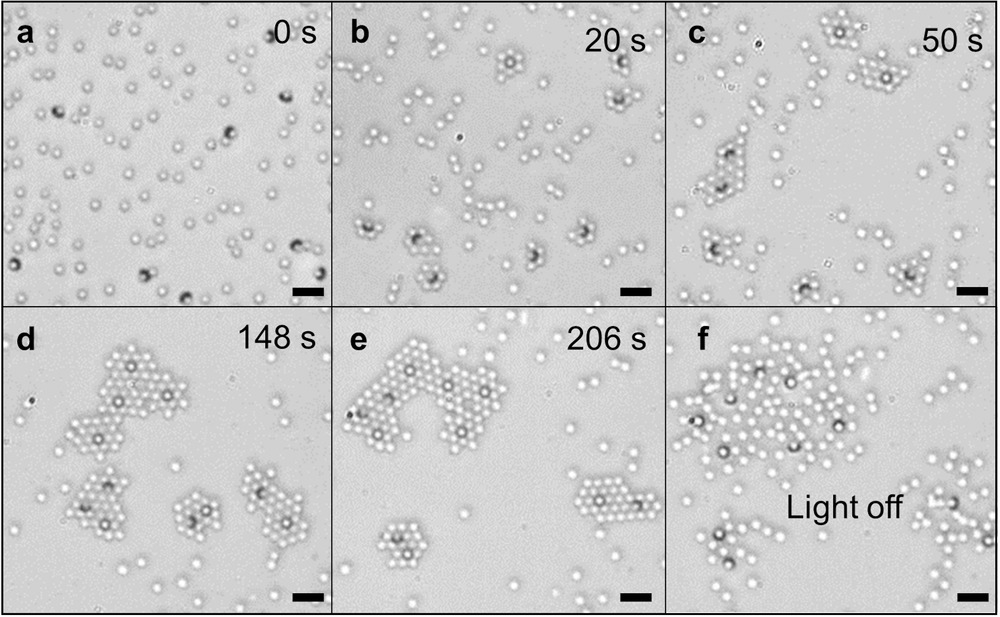
\includegraphics[width=0.7\textwidth]{singh-particles.jpg}
\end{figure}

\subsection{Why active matter?}

The cool thing for me about active matter is that it aims to study many particle systems far from equilibrium where scaling geometrical properties and phase transitions are also shown to occur.

\section{Viseck Model and Flocking}

Very cute model! Very simple and exhibits kinetic phase transition! :D

The Viseck model describe the motion of driven particles subject to some noise. 

Initially, $N$ particles are placed in a box, randomly distributed, with the same absolute velocity $v$ and with randomly distributed directions $\theta$. The position of the $i$-th particle is updated at each time step by:
%
\begin{equation}
	\mathbf{r}_i(t+\Delta t) = \mathbf{r}_i(t) + \mathbf{v}_i(t)\Delta t,	
\end{equation}
%
where the velocity has always the same absolute value $v$ and an orientation given by:
%
\begin{equation}
	\theta(t+\Delta t) = \langle\theta(t)\rangle_r + \Delta \theta,
\end{equation}
%
and $\langle \theta(t)\rangle_r = \arctan[\langle \sin(\theta(t))\rangle_r /\langle \cos(\theta(t))\rangle _r ]$ is the average orientation of the velocity of all the particles within a circle of radius $r$ around the $i$-th particle (including itself). $\Delta \theta$ represents noise and is a random number chosen with uniform probability from the interval $[-\eta/2,\eta/2]$.

This system has three free parameters:
%
\begin{itemize}
	\item $\eta$ the maximum angle of the distribuition
	\item $\rho$ the density of particles
	\item $v$ the absolute velocity of the particles (which remains constant thorughout the experiment).
\end{itemize}
%
In his work, Vicsek used $0.003<v<0.3$ since a small velocity would correspond to the limit of stationary particles (i.e. the XY model) and two high velocities would make the particles become mixed between two updates, and this limit corresponds to the so-called mean-field behaviour of a ferromagnet.

\subsection{Results/Behaviours}

\begin{itemize}
	\item At t = 0 the positions and the direction of velocities are distributed randomly.
	\item For small densities and noise the particles tend to form groups moving coherently in random directions.
	\item At higher densities and noise the particles move randomly with some correlation. 
	\item Perhaps the most interesting case is when the density is large and
 the noise is small; in this case the motion becomes ordered on a macroscopic scale and all of the particles tend to move in the same spontaneously selected direction.
\end{itemize}

\subsection{Phase-Transition emerges}

In this sytem, the total momentum is not conserved. The interactions here work through the averaging of the particle orientation of adjacent particles. It turns out, that in this case, we can define an order parameter, which is the absolute value of the average noramlized velocity:
%
\begin{equation}
	v_a = \frac{1}{Nv}\vert \sum_{i=1}^N \mathbf{v}_i \vert
\end{equation}
%
this velocity is $\approx 0$ for randomly oriented velocities and $v_a\approx 1$ when all the velocities are closely aligned.

By changing the density of particles $\rho= N/L^2$ and the noise $\eta$, a difference in the behaviour of $v_a$ was observed - \textbf{phase transition:}
%
\begin{figure}[H]
	\centering
	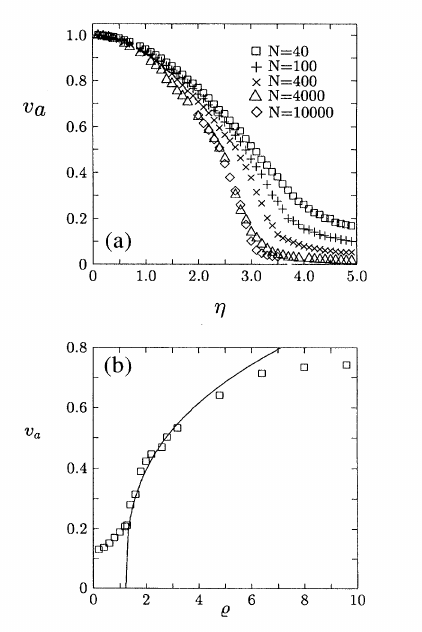
\includegraphics[width=0.4\textwidth]{vicseck-phase-transition.png}
\end{figure} 
%
and they were also able to estimate the critical exponents and make analogies to the ferromagnetic case; the noise plays the role of temperature (makes sense) and the density the density of spins. They follow the laws:
%
\begin{align}
	v_a \sim [\eta_c(\rho)-\eta]^\beta && v_a \sim [\rho-\rho_c(\eta)]^\delta
\end{align}
%
with  $\beta = 0.45 \pm 0.07$ and $\delta = 0.35 \pm 0.06$.

Also, for the noise we have:
%
\begin{align}
	\langle \eta_i(t) \rangle = 0 && \langle \eta_i(t)\eta_j(t')\rangle= 2\gamma \delta_{ij}\delta_{tt'}
\end{align}
%
(meaning, white noise :p).


\section{Mermin-Wagner Theorem}

Why is the Vicsek model important or interesting? It is \textbf{intrinsically non-equilibrium} and it exhibits a phase transition. This would not be possible for 2D models in equilibrium due to the Mermin-Wagner theorem.

The argument is simple. We take our Vicsek model and take the case where the modulus of the velocity is zero. Then we simply have a system of oriented spins in space, also known as the Heisenberg model. Next, we assume that, for finite temperature, there is an orientation of the spins in a given direction. Assuming the preferential direction of alignment is in the $x$ direction, we can write that out as:
%
\begin{align}
	\mathbf{S} = (\sqrt{1-\sigma^2}. \sigma, \sigma, \cdots)
\end{align}
%
where $|\sigma| \ll 1$. These are our perturbations, or Goldstone modes, that arise as low frequency (high wavelengths) perturbation for finite temperatures close to zero. 

From this, it is possible to show that the fluctations would diverge for $d\leq 2$, hence, the initial assumption that the system is in a preferential alignment would be broken. Hence, there can be no phase transition in these systems for less than 3 dimensions. A nice heuristic argument for this fact is given by John Cardy (Scaling and Renormalization in Statistical Physics):

\textit{For systems with a continuous symmetry, however, the energet-energetics of domain walls is quite different. If we form a domain of size $l$ by insisting that the spins near the centre of the domain point inthe opposite direction from those far away, then the interveningspins have a distance $O(l)$ over which to relax. Since they may do this in a continuous fashion, the relative angle between two neighbouring spins will be $O(1/l)$, and the energy density of sucha configuration is $O((1/l)^2)$. This yields a total energy $O(l^{d-2})$ for a domain whose volume is $O(l^d)$, as compared with $O(l^{d-1})$ in the discrete case. This means that the entropic effects will always win for $d\leq 2$.
}

Hence, in a system at equilibrium, flocking would not happen in two dimensions.


\section{ABPS theory, phase diagram, etc}

\subsection{Active Brownian Particles (ABPs)}

Let us begin by review what is a "regular brownian particle", or should we say, a particle subject to thermal fluctuations in equilibrium.

\subsubsection{Brownian Motion}
\paragraph{Feynman's Notes} 

The Brownian movement was discovered in 1827 by Robert Brown, a botanist. He noticed particles of plant pollens in a liquid and realised it wasn't a living being. He also found particles in water trapped inside a quartz crystal for millions of years. The cause of this motion was molecular motion to the temperature.

``
we have been perpetually making a certain important assumption, which is that if a given system is in thermal equilibrium at some temperature, it will also be in thermal equilibrium with anything else at the same temperature.
''

 The reader may easily verify that the number of collisions a single molecule of water receives in a second is about 1014, so in a hundredth of a second it has 1012 collisions, which is a lot! Therefore, after a hundredth of a second it is not going to remember what happened before. In other words, the collisions are all random, so that one “step” is not related to the previous “step.”
 
 (this is exactly the condition for a Markov process)

The sailor is making some relatively sensible headway, but only such that his mean square distance is proportional to time. That is the characteristic of a random walk.
 
If the drunken man takes $N$ steps of length $L$ it is easy to prove that the mean displacement squared
$<\mathbf{R}^2> = NL^2$.

It was actually Einstein and Smoluchowski that were able to determine how far a particle would be displaced after a time t, with brownian motion. The math is very cute. We begin with Newton's law with some damping:

\begin{equation}
	md_t^2x + \mu d_t x = F
\end{equation}

where $\mu$ is the drag coefficient that we can measure experimentally. Then, we can take the averages. Recall that we want to calculate $d_t<\mathbf{r}^2>$ . Let's begin by $<x^2>$ since $<\mathbf{r}^2>=3<x^2>$ (since the motion is random there is no prefered orientation). So, rewritting newton's equation and multiplying it by $x$ we get:

\begin{align}
	xm\frac{d^2x}{dt^2}+\frac{\mu}{2}\frac{dx^2}{dt} = xF\\
	\Leftrightarrow m\left(\frac{d}{dt}\left(x\frac{dx}{dt}\right)-\left(\frac{dx}{dt}\right)^2\right) +\frac{\mu}{2}\frac{dx^2}{dt} = xF
\end{align}
%
We can now average out both sides of the equation. Both of the terms that are multiplying by $x$ disappear, because x can take any positive or negative values. Since the motion is random, there is no reason why the force or the velocity should be in the same direction as $x$ (there is no memory of the past), so they can also go in either positive or negative direction, hence, in the end, those terms average out to zero. The second term simply corresponds to the average kinetic energy. Hence, we get:

\begin{equation}
	\frac{d\langle x^2\rangle }{dt} = \frac{2k_BT}{\mu} \implies \langle \mathbf{r}^2\rangle = 6\frac{k_BT}{\mu} t.
\end{equation}

The MSD goes linearly with $t$. This is a \textbf{diffusive behaviour}.

\textbf{Memory is an important aspect.} When we say Brownian motion occurs due to thermal fluctuations, we refer to the collisions that exist between the atoms in a mixture that carry the particles. As we saw, molecules are constantly being bombarded by atoms in absurd amounts. There are so many collisions that we lose track of it's \textbf{history}. There is no \textbf{preferential direction of flow}, no \textbf{transport}, IE, the \textbf{linear and angular momentum} remain constant over time! And the energetic contribuitions from the linear and angular motions add up to the value predicted by the equipartition theorem.

\subsubsection*{Einstein's Deduction}

Let us call $q$ the distance increment of a particle in a time $\tau$ and the density of particles $\rho(x,t)$. This increment is modeled by a probability distribuition $\varphi(\tau)$. Expanding the density in a Taylor series we get:

\begin{equation}
	\rho(x,t+\tau) = \rho(x,t) +  \tau \frac{\partial \rho(x,t)}{\partial t} + \cdots
\end{equation}

We can also write out the particle density at a point $x$ at time $t+\tau$ by taking the probability of a particle being in $x-q$ at time $t$ and integrating over all probabilites:

\begin{align}
	\rho(x,t+\tau) &= \int_{-\infty}^\infty \rho(x-q,t)\varphi(q)dq \\
	&= \int_{-\infty}^\infty \left(\rho(x,t)\varphi(q) + \frac{\partial \rho}{\partial x} (-q)\varphi(q) + \frac{\partial^2\rho}{\partial x^2}q^2\varphi(q) + \cdots\right) \\
	&= \rho(x,t)\int_{-\infty}^\infty \varphi(q)dq - \frac{\partial \rho}{\partial x} \int_{-\infty}^\infty q\varphi(q)dq + \frac{\partial^2\rho}{\partial x^2}\int_{-\infty}^{\infty} q^2\varphi(q)dq + \cdots \\
	&= \rho(x,t) + \frac{\partial^2\rho}{\partial x^2} \underbrace{\int_{-\infty}^\infty q^2\varphi(q)dq}_{\tau D \textrm{where, $D$ is the mass diffusivity}} + O(\textrm{other even contributions})
\end{align}

Hence:

\begin{align}
	\frac{\partial \rho}{\partial t}=D\frac{\partial^2 \rho(x,t)}{\partial x^2}
\end{align}

which, for $N$ particles it has a gaussian solution:

\begin{equation}
	\rho(x,t) = \frac{N}{\sqrt{4\pi Dt}}\exp\left(-\frac{x^2}{4Dt}\right)
\end{equation}
%
with a variance $\sigma^2= 2Dt$, first moment $\langle x \rangle = 0$ and second moment $\langle x^2 \rangle = 2Dt$, proportional to the diffusive constant and the time.

Then I can add a simulation of a browninan particle.

The simplest way to model a brownian particle is in the overdamped regime where the equation of motion is given by:

\begin{equation}
	\gamma\frac{d \mathbf{r}}{dt} = -\nabla U + \mathbf{\Gamma}(t)
\end{equation}

\subsection{Active Brownian Particle (ABP)}

Active Brownian Particles are generalisations of brownian particles to a nonequilibrium system. These particles exhibit self-perpulsion, on top of the dissipative environment. In the simplest model, we think that the particles have a random oriented active velocity applied to the center of mass. Both the orientation and translation are subject to random fluctuations:

\begin{equation}
	\gamma \frac{d \mathbf{r}}{dt} = -\nabla U + \Gamma(t) + \mathbf{F_a}
\end{equation}

The orientation is usually given by a normalized vector $\mathbf{n}_i = (\cos \theta_i(t),\sin \theta_i(t))$ for each particle $i$. Then, the equations of motion look something like this:

\begin{align}
	\gamma \dot{d\mathbf{r_i}} = F_\text{act}\mathbf{n}_i - \nabla_i \sum_{(i\neq j)} U(r_{ij}) + \sqrt{2\gamma k_B T}\xi_i,\qquad \dot{\theta_i} = \sqrt{2D_\theta }\eta_i
\end{align}

For the potential, we usually consider two different types of potentials, either a cut and shifted LJ potential:

\begin{align}
	U(r)=
	\begin{cases}
		U_{LJ}(r)-U_{LJ}(r_\text{min}) \quad \text{if} \quad r<r_\text{min}\\
		0 \quad \text{if} \quad r\geq r_\text{min}
	\end{cases}
\end{align}

The random noise is, in the simplest case, to be considered white noise:

\begin{align}
	\langle\eta_i(t)\rangle= 0,\quad \langle \eta_i(t)\eta_j(t')\rangle = \delta_{ij}\delta(t-t')\\
	\langle\xi_i(t)\rangle= 0,\quad \langle\xi^\alpha_i(t)\xi^\beta_j(t')\rangle=\delta_{ij}\delta^{\alpha\beta}\delta(t-t')
\end{align}

and the diffusive constant is $D_\theta= 3k_B T/\gamma \sigma_d^2$, where $\sigma_d$ is the radius of the particles. (\textcolor{red}{where does this come from?}). Other things that are useful to us are the definitions of packing fraction and activity (Péclet number):

\begin{enumerate}
	\item $\phi_p = N\frac{\pi \sigma_d^2}{4S}$ (S is the total surface, this is essentially a measure of the density of particles) in the 3D case we have $\phi=N\frac{\pi \sigma^3}{3V}$, where $\sigma$ is the diameter (we needed a length scale here and it's the diamater because it's the standard in LAMMPS).
	\item $\text{Pe}=\frac{L v_\text{act}}{D}=\frac{\sigma_d F_\text{act}}{K_B T}$. It is defined as the ratio between active transport and diffusive transport. So, usually,
	$
	\text{Pe} = \frac{\text{active transport}}{\text{diffusive transport}}
	$
\end{enumerate}

Another useful potential is the Mie potential, which takes care of the cut in the LJ potential:

\begin{equation}
	U_\text{mie}=4\epsilon\epsilon_0\left[\left(\frac{\sigma_\text{Mie}}{r}\right)^{2n}-\left(\frac{\sigma_\text{Mie}}{r}\right)^{2}\right]\theta(r_c-r)-4\epsilon\epsilon_0\left[\left(\frac{\sigma_\text{Mie}}{r_c}\right)^{2n}-\left(\frac{\sigma_\text{Mie}}{r_c}\right)^{2}\right]
\end{equation}

Where we essentially have a hard core repulsion.

\textcolor{blue}{Open questions:
\begin{enumerate}
	\item the formula for the $D_\theta$, it seems to also come from the fluctuation dissipation theorem?
	\item animations for the active and passive particles (I can still but I think it's more instructive to do my own)
\end{enumerate}}

\section{Interesting papers on the active matter systems}

\subsection{Athermal Phase Separation of Self-Propelled Particles with No Alignment - 2012 Fily and Marchetti}

\textbf{Abstract}

This paper is a study of a system of 2D self-propelled disks, with isotropic repulsion forces and rotational noise. There is no aligning interaction, which the authors claim to be why there is no ordered state. They notice large number fluctuations and cluster formation as is found in active systems. They argue that these results are characteristic of systems that are locally driven out of equilibrium like, in this case, by self-propulsion.

\textbf{Introduction}

Collective self-propelled particles are perhaps the simplest model for active particles - class of nonequilibrium systems composed of individual units that that consume energy and collectively generate motion or mechanical stresses. They encompass large length scales, from the cell cytoskeleton, to bacterial colonies, to school of fishes to tissues and animal groups. - they exhibit phase separation, swarming, pattern formation, anamolous fluctuations, etc.

For systems in equilibrium away from a critical point, the number fluctations grow was $Delta N \propto \sqrt{N}$, but in active systems they grow as $\Delta N \propto N^\alpha $, where $\alpha$ can go up to 1 in 2D. This is true for both nematic and polar states. (In nematic, though the orientation between particles is paralel, but it doesn't point in one of the directions, while for polar it does). The authors believe the number fluctiations are associated with broken rotational symmetry!

They found that there is no \textbf{large scale alignment} rule as is found for systems of rods that exhibit nematic ordering.  They did find, is that after a packing fraction of 0.4, large clusters begin to form. There is a sort of phase separation between a gas like and a solid like states. The system exhibits huge number fluctuations. They believe that the cause for this phase separation is not a broken rotational symmetry like in the rods system, but rather because the rate at which the particles diffuse is smaller than that the length scale for the configuration/arrangement of disks to entrap others. They call this steric entrapment. The authors thus argue that this behaviour comes from the fact that the system is locally driven out of equilibrium and detailed balance is broken by a persistent energy input (the self propulsion). They also argue that the system cannot be described as having an "effective temperature"

\textbf{Body}
The simulation is done very similarly to the Viseck model, but here, the velocity also comes from the interactions with the colliding particles. Momentum is not conserved!\\

They observe large clustering even without alignment and anisotropic particles. So it must only be due to the nonequilibrium dynamics. Aditionally, An equilibrium thermal system cannot replicate the results, as was suggested by some authors. The authors of this study argue that that may only be done in very dilute systems.

They find giant number correlations with $\Delta N \propto N^\alpha$ and they find that the orientational correlations vanish (only some remain at the border of the clusters, pointing inwards), so its not orientational order that causes cluster formation.

MSD - can be modeled with as persistent random walk and an effective velocity of the particles calculated. it is ballistic for short times and diffusive for larger times. with increasing packing fraction the ballistic behaviour lasts less.

They describe a continuum model. 

\subsection{Structure and Dynamics of a Phase-Separating Active Colloidal Fluid - 2013 - Redner, et al.}

This is essentially a generalisation of the previous work but with 3D spheres. Besides the phase separation, they also so that the system undergoes a continuous phase transition analagous to equilibrium systems with attraction interactions. There is phase-separation kinetics and it is possible to discern between different phases. There is also equilibrium-like coarsening. They also find the existance of a new "active solid" phase, that exhibits structural properties consistent with a 2D colloidal crystal near the crystal-hexatic transition point.

Similar to the previous article, the system is made up of spherical particles enclosed in a fluid and the only interaction between particles is that of an isotropic excluded-volume repulsion only. 

They found, just as the 2D case, that that above certain Pe numbers and packing fraction, the system would form clusters. Aditionally, the authors were able to identify a binodal envelope beyond which the system separates into two phases whose density colapses into a single coexistance curve, which is a function of activity alone. This suggest the system behaves as an equilibrium system of mutually attracting particles undergoing a phase transition. This contradicts the intuitive idea that activity will disrupt the system. \textbf{key idea here!} They found a critical point at the apex of the binodal curve, with $\phi_p=0.7$ and Pe=50.

The Phase-separated steady state. The authors measured the fraction of particles in the dense state and verified that it was a non trivial function of the activity and packing parameters. To understand this relation they developed a kinetic model. They assumed that the particles in the cluster were trapped and modeled a stationary state where gas particles in contact with the cluster are automatically absorbed and that particles within the cluster can become free if their velocity orientation lies above the horizon. From the steady state equation (flux of particles coming in = flux of particles coming out) they are able to determine the shape of the binodal curve, using a free parameter $\kappa$, the number of particles of particles lost per escape event of the cluster.

The structure of the dense phase. Inside the cluster there is, at low Pe, a liquid-like isotropy, but as activity is increased, the phase starts developing a strong six-fold symmetry. The density distribuition function reveals clear peaks at the vertices of an hexagon, as it is also shown by the correlation function. \footnote{ More generally, a hexatic is any phase that contains sixfold orientational order, in analogy with the nematic phase (with twofold orientational order).}. This material is unique in that it is held together by active forces alone, and that the arrest of motion is due to frustration. In this sense it is similar to amorphous materials such as granular packs as reflected by the highly heterogeneous stress distribution. They also observe that there are defects inside of the clusters.

The dynamics of the solid phase. They measured the MSD inside the cluster and found that, though individual particles had diffusive, ballistic and diffusive behaviour (in short, medium and long timescales), the whole of the cluster had sub-diffusive, diffusive and superdiffusive behaviour.

As far as the phase separation kinetics are concerned, although the system undergoes an athermal phase transition, the parameters of packing fraction and activity can be tweaked to inducing a sort of quenching effect. Systems quenched close to the binodal exhibit a nucleation delay which can be long enough that artificial seeding is necessary for phase separation to be computationally accessible. Systems quenched more deeply undergo spinodal decomposition, leading to a coarsening regime in which the mean cluster size scales surprisingly as $t^{1/2}$, with a corresponding length scale of $t^{1/2}$.

\subsection{Full Phase Diagram of Active Brownian Disks: From Melting to Motility-Induced Phase Separation - 2018 - Digregonio et al}

\textbf{Abstract}

Self-propelled hard disks in 2D, they are able to show the full phase diagram, have an equation of state. The equilibrium melting scenario is maintained at small activities, with coexistence between active liquid and hexatic order, followed by a proper hexatic phase, and a further transition to an active solid. As activity increases, the emergence of hexatic and solid order is shifted towards higher densities. Above a critical activity and for a certain range of packing fractions, the system undergoes motility-induced phase separation and demixes into low and high density phases; the latter can be either disordered (liquid) or ordered (hexatic or solid) depending on the activity.

\textbf{Introduction}

Other than the usual stuff they mention that a hallmark of active particle systems is that for high enough density and activity , the self-propulsion triggers a motility induced phase separation (MIPS) into a low density gas phase in coexistance with a high-density drop. This resembles equilibrium liquid-gas transitions \textbf{but} in the absence of cohesive forces and without thermodynamical support.

In this letter the authors address the melting in a 2D system of self-propelled disks and study what happens as the Pe tends to zero. . They indicate that melting of passive hard disks takes place in two steps: as the packing fraction is increased, a first-order transition between the liquid and hexatic phases occurs, followed by a continuous Berezinskii-Kosterlitz-Thouless (BKT) transition between the hexatic and the solid. The hexatic phase exhibits quasi-long-range orientational order and short-range positional one, while the solid phase has quasi-long-range positional and long-range orientational order.

\textbf{Phase Diagram}

A phase diagram for packing fractions up to close packing $\phi_{cp}\approx 0.91$.

\begin{itemize}
	\item They verify the behaviour that is known for passive particles at Pe$\sim 0$. There is a melting with two phase transitions, with a coexistance between active liquid and hexatic phases. 
	\item Above Pe=1, an active hexatic order exists for all explored activities and at a wider density range.
	\item At higher densities there is quasi-long-range positional and orientational long-range order for all activites, signaling the presence of an active solid.
	\item The hexatic-solid and liquid-hexatic transitions shift to higher densities with activity - activity disturbs order.
	\item There is a coexistance region at high activities. MIPS prevails over hexatic and solid phases for high activity. There are separations between dilute and high-density phase.
\end{itemize}

\textbf{Equation of state}

The authors were able to write out an equation of state $P(\phi)$, which is the mechanical pressure and which helps them estimate the phase boundaries. They calculate: $\Delta P = P - P_\text{Ideal Gas} = P_\text{active} + P_\text{particle interactions}$.

With the equation of state for the low Pe regime, they were able to identify a coexistance area and double loop mattern in P VS $\phi$ that matches the phase diagram. They were able to determine the width of the coexistance area by a Maxwell construction (as a first approximation because there are other works that question that generalisation). They do not find evidence of coexistance until the MIPS region for Pe$\geq$ 35. At this point, the curves become flat. for a hider area. The limits of the MIPS are calculated from the spinodal for Pe=100. It can also be done looking at the PDFs, they also found the double peak structure there.

For the coexistance phase, the system acquires ideal gas pressure, because the interactions cancel out the pressure resulting from the active force.

\textbf{Orientational order and hexatic phase}

Next, to study the transition, they studied the correlation function of the hexatic order parameter and also studied the kurtosis or Binder parameter.

The behaviour of $g_6$ is:

$$
\begin{cases}
	\text{exponential - active liquid}\\
	\text{algebraic - active hexatic}
\end{cases}
$$

and the exponent for the algebraic behaviour matches that predicted by the BTK (hexatic-solid) transitions that exists for passive particles. The binder cumulant behaviour also confirms the phase boundaries found with this method.

Furthermore, the authors note: ``a weak remanent N dependence that would be compatible with a first order phase transition [46,47]; however, the accuracy of our data is not enough to draw such a conclusion and, moreover, a second order transition is consistent with the absence of phase coexistence found above Pe $\approx$ 3. As illustrated in Fig. 3(b), activity shifts the emergence of orientational quasi-longrange order to higher densities."

\textbf{Orientational Order and coexistance}

We saw that there are 2 regimes of coexistance of low and high density regions, one for low Pe and another one at high Pe. The difference in these regimes was analised by the authors with PDFs analysis.

At low Pe: The pdfs show a binodal regime, with equally sized density peaks. Furthermore, there is a system sized ramifies region all with the same orientational order.

At high Pe: The pdfs show a smaller peak at lower $|\Psi_{6j}|$ and higher one at high $|\Psi_{6j}|$ (borders between different regions of almost perfect orientational order). There are several regions that are more like blocks. With higher orientational order within each region and quasi-long positional order - there are several regions with different orientations.

\textbf{Positional order and the solid phase}

They could not say for sure whether $g_6$ acquires long-range order or does not decay at length scales of the size of system and could decay into a larger distance, so they looked for solid quasi-long range positional order, but studying the first peak of the structure factor:

$$
C_\mathbf{q_0}(r) = <e^{i\mathbf{q_0\cdot (r_i-r_j)}}>
$$

There is a change in behaviour from exponential (hexatic) to algebraic (solid) that allowed the authors to draw the transition curve.

Activity introduces non-equilibrium fluctuations that destabilize order and melt the solid.

\textbf{Conclusions}

\begin{itemize}
	\item the theory of melting passive disks with 2 transitions is still valid for low activity (Pe $leq$3);
	\item weakn activity acts as a perturbation that distabilizes passive order. This is seen by 1) the shift in the liquid-hexatic and hexatic-solid transitions for higher densities with higher Pe and 2) by the shrinking and eventual disapearence of the coexistance phase. In equilibrium particle softness has these effects, so the authors argue that activity acts as an \textbf{effective softness} - $\Gamma = \varepsilon/(\sigma_D F_\text{act})$
	\item At high Pe, the MIPS reagions appear, and hexatic and solid phases still prevail. In these cases there are several patches of highly oriented regions that recombine and merge together, a behaviour different from the one found at lower Pe
	\item for dumbells it had been found before that the regions of coexistance were continous in the phase diagram, this is not true here. This suggests that the geometry has a role in the behaviour of the particles.  The \textbf{nonconvex geometry} of the dumbells could ease jamming and the formation of local orientational order.
\end{itemize}

\section{KTHNY Theory and other results that arise from this discription of active particles}

This is useful to understand the results of the active disks and active spheres. This is a theory for the melting of crystals in 2D, where the authors argue that the system undergoes 2 different phase transitions, one from liquid-hexatic and another from hexatic-crystal. The phases are characterised by their strucutre factor and correlation coefficients. Let's dwelve into it!

- it can be soilved analytically and exhibits a phase transition for T>0.

- this theory predicts the unbinding of topological defects to break the symmetry in two steps at two distinct temperatures. Dissociation of dislocation pairs first
melts the crystal into a still orientational ordered (hexatic) phase and, in the second step,
dissociation of free dislocations causes the system to go isotropic fluid.

- we generaly see symmetry breaking in phase transitions when we lower the temperature. this is true for solids melting into liquid and gas (there is positional and rotational symmetry at these high temperature states, it is equally likely to be anywhere in the system, they are isotropic as well). This also happens in the para-ferromagnetic phase, there the spins go from randomly oriented (rotational symmetry) to being align in a certain dimension, as the temperature lowers. The free energy is reduced with the decrease in temperature and increase in order: F=U-TS, so the internal energy drops as well.

-  As a general
concept, during heating of the system, increasing amounts of defects in the ordered phase and
dynamical (vibrational) modes provide the tools to restore symmetry.

- It is hard to study these systems, a lot of times we have to deal with singularities (like jumps in the specific heat) -$>$ development of phenomenological theories, that show that microscopic interactions are not as important. This happens because of large fluctuations in the order parameter - these systems can be described into universality classes regardless of microscopic properties.

\subsection{2D}

For 2D, no long-range order exists, due to long wavelength fluctuations. 

- Melting is driven by the emergence
- in the crystalline phase - of a class of topological defects, namely thermally activated dislo-
cations pairs which dissociate at the melting temperature Tm (Kosterlitz and Thouless 1973;
Young 1979). This gives rise to a softening of the crystal’s compressibility and shear elas-
ticity and the melting transition is a second order transition. 

\textbf{Basic characteristics of the KTHNY Theory}

\begin{enumerate}
	\item Unlike 3D, in 2D there is a fourth state of matter between liquid and solid. Initially it was thought that between liquid and solid there were 2 distinct 2nd order transitions, now people think there is rather a 1st order transition and a 2nd order transition
	\item These transitions arise from the emergence of collective topological defects, and also come from the fact that in 2D, the system cannot escape fluctuations, so 2D is more vulnerable and different symmetries are broken.
	\item There are several ways we can quantify the existance or not of an hexatic phase
\end{enumerate}

\subsection{Checking the predictions of the KTHNY}

\paragraph{Two-point radial correlation function:}

\begin{equation}
	G(\mathbf{r}-\mathbf{r'}) = \langle\rho(\mathbf{r})\rho(\mathbf{r}')\rangle-\langle\rho(\mathbf{r})\rangle\langle\rho(\mathbf{r}')\rangle
\end{equation}

\paragraph{Order parameter}

\begin{equation}
	\psi_6(j)=\frac{1}{N_c}\sum_{k=1}^{N_j}e^{i6\theta_{jk}}
\end{equation}

where $N_c$ is the number of clusters, and for each cluster we are checking the orientation with others according to a defined reference axis.

\paragraph{Orientational Order Parameter}

\begin{equation}
	\psi_6 = \lvert \frac{1}{N_c}\sum_{j=1}^{N_c}\psi_6(j) \lvert
\end{equation}

and the associated susceptibility:

\begin{equation}
	\chi_6 = N_c \left(\langle \psi_6^2\rangle -\langle\psi_6\rangle^2\right)
\end{equation}

\paragraph{Two point orientation correlation function:}

\begin{equation}
	g_6(r)=\langle\psi_6(j)\psi_6(k)\rangle
\end{equation}

But Giuseppe actually defined this as:

\begin{equation}
	g_6(r)=\frac{\langle\psi_6(j)\psi_6^*(k)\rangle_{r_{jk}=r}}{\langle\lvert\psi_6(j)\lvert^2\rangle}
\end{equation}

Which is basically equivalent. We are taking a correlation over all the orientations of the clusters and then we are normalizing it.

In short, the solids first break apart into clusters through a process called dislocation unbinding. This is the hexatic state, where there is still some quasi-long range orientational order. The particles walk around with not exactly 6 neighbours as would be expected for the cristaline phase, so we don't see dirac deltas in the structure factors. Later, the disclination unbinding occurs, and the phase transition for a fluid.

\url{https://gpantel.github.io/analysis-method/2D\_boo/}

A main question remains: \textbf{this is true for systems in equilibrium. What about systems out of equilibrium? Does this theory also generalises for active systems? And will we observe hexatic states in 3D?}

\section{Defect mediate phase-transitions (Nelson)}

There were some advances in equilibrium statistical mechanics and defects in phase transitions when scientists in the 70's started studying 2D systems in equilibrium with topological defects. The most impressive novelty that might have come from this is the existance of a fourth state of matter, the hexatic state.

There exist two broken symmetries separating low-temperature solids and high temperature fluids. Going from liquids to solids, we know that the translational invariance of a fluid is broken by the regular patterns of crystals that we see in Bragg peaks. Breaking the translational invariance implies a \textbf{long-range orientational order}. 

An intermediate phase, the hexatic phase, consists of a short-ranged positional order but a broken rotational symmetry that is associated with bonds between different molecules. This state exhibits a residual 6-fold symmetric diffraction pattern and a vanishing shear modulus.

This hexatic phase as been found in liquid-crystal films, in colloidal crystals, in magnetic bubble arrays and also in 3D in stacked layers of smectic LC in dense solutions of DNA and in flux line arrays of high-temperature superconductors.

When know that for dimensions inferior to 4, the mean-field values of the critical exponents are shifted close to phase-transitions due to the effects of the fluctuations.

Consider the equilibrium correlation functions:

\begin{align*}
	G(r) = \langle \psi(\mathbf{r})\psi^*(\mathbf{0})\rangle \\
	 = \langle \rho_G(\mathbf{r})\rho_G^*(\mathbf{0})\rangle \\
	  = \langle \mathbf{S}(\mathbf{r})\mathbf{S}^*(\mathbf{0})\rangle  
\end{align*}

where $\psi$ is the comlex wave function of a superfluid, $\rho$ is the local Fourier component of the mass or number density of a crystal  at the reciprocal lattice vector $\mathbf{G}$.

If there is no long-range order, like in a liquid, in a paramagnet or in the normal phase of a superfluid, the correlation falls exponentially:

\begin{align*}
	G(r)\sim e^{-r/\chi(T)}
\end{align*}

where $\chi(T)$ is a temperature-dependent correlation length. If a symmetry is broken, then the correlation will tend towards a constant for large $r$:

\begin{align*}
	\lim_{r\rightarrow \infty} G(r)=\text{constant}\neq0
\end{align*}

In a superfluid, this means that the phases of the wave function add up coherently from point to point, and in a magnet, the magnetizations points in a definite direction.
Long range order in crystals represents broken continous translational symmetry and shows up as delta-dirac functions in bragg peaks in the X-ray structure factor. There can also be broken \textit{orientational} symmetry represented by singled out crystallographic axes. The correlation function can also decay algebraically to zero,

\begin{align*}
	G(r)\sim 1/r^{d-2+\eta}
\end{align*}

where $d$ is the dimension of the system and $\eta$ a critical exponent. This decay happens for 2nd order phase transitions. Since melting in 3D is usually a 1-st order transition, this decay doesn't usually happen in 3D.

In 2D, the long-range correlation behaviour is impossible, because the system has to few dimensions to handle the fluctuations (and Goldstone modes?). Instead, it is observed a power low behaviour with an exponent that depends on the temperature:

\begin{align*}
	G(r)\sim 1/r^{\eta(T1)}
\end{align*}

The formation of the hexatic ordering in 3D has been hardly understood – according to the Halperin and Nelson theory1 the hexatic phase arises as a consequence of the broken translational symmetry of a 2D crystal, induced by dissociation of thermally excited dislocation pairs. The transition to an isotropic liquid occurs only after a subsequent unbinding of the disclination pairs. Such a defect-mediated mechanism clearly does not work in 3D crystals due to the difference in defect formation energies in the 2D and 3D cases. Fortunately, the hexatic phase in LCs can be fully described on the basis of symmetry considerations, which does not imply any specific melting mechanism.

\section{Marenduzzo's paper on the 3D abps }

In this paper there is no immediate evidence of an hexatic phase. The spinodals were drawn by visual inspection and by fitting the power-law growth of the domain sizes.

\section*{Other things I want to learn more about}

\begin{enumerate}
	\item fluctuation dissipation theorem - I think I finally managed to learn more about this! Rosa's notes are incredible! I have some notes on paper as well :D
	\item what is a spinodal decomposition - Spinodal decomposition is a mechanism by which a single thermodynamic phase spontaneously separates into two phases (without nucleation).[1] Decomposition occurs when there is no thermodynamic barrier to phase separation. As a result, phase separation via decomposition does not require the nucleation events resulting from thermodynamic fluctuations, which normally trigger phase separation. 
	\item what is a binodal - In thermodynamics, the binodal, also known as the coexistence curve or binodal curve, denotes the condition at which two distinct phases may coexist. Equivalently, it is the boundary between the set of conditions in which it is thermodynamically favorable for the system to be fully mixed and the set of conditions in which it is thermodynamically favorable for it to separate into two phases.[1] In general, the binodal is defined by the condition at which the chemical potential of all solution components is equal in each phase.
\end{enumerate}

\begin{figure}[H]
	\centering
	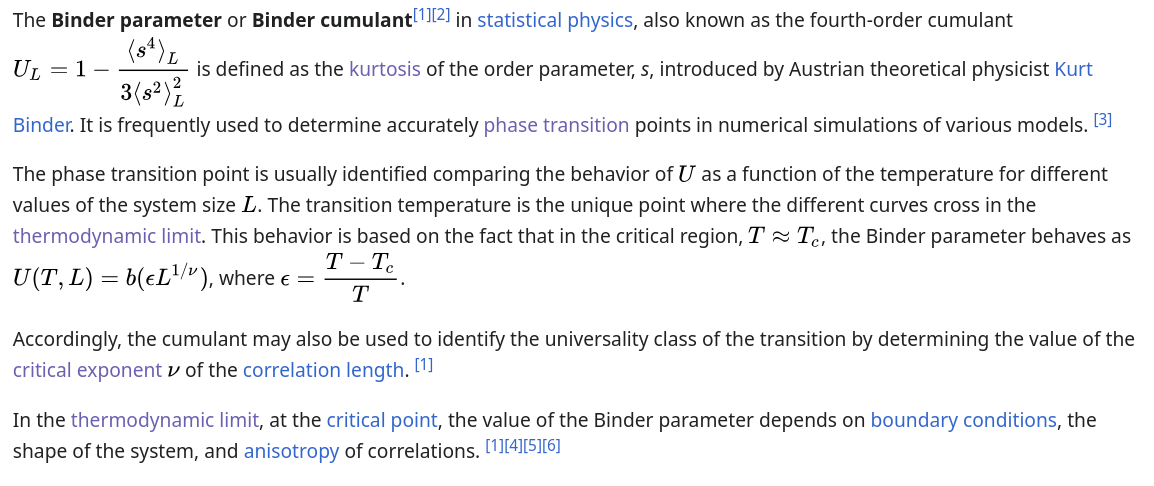
\includegraphics[width=\textwidth]{binder-cumulant.png}
\end{figure}

\section{Prepare the presentation}

Idea - Over all these years we have built the theory of statistical physics of equilibrium. But there are a lot of interesting systems that exists out of equilibirium. How can we study those? What kind of things to we observe? Is it possible to generalise the knowledge and tools we have from equilibrium physics to systems out of equilibrium?

Why are these systems interesting? What is active matter? What are the main distinctions from passive matter?

\begin{itemize}
	\item a comparison between passive and active particles
	\item how to simulate these particles
	\item what sort of new behaviours emerge from it
	\item how to characterize these states of matter and what do we find in them
	\item what critical phenomena do we find in these systems?
	\item what are open questions that need to be addressed?
\end{itemize}

\subsection{Plan}

\begin{itemize}
	\item introduce the concept of active matter in different scales, from inside cells to colonies of cell and up to flocking and other behaviours
	\item Top-down approach, start with the viseck model and go from there (also check Parisi maybe?)
	\item From the flocking go into the active particles
	\item finish with the particular papers
\end{itemize}

\subsection{Advices}

\begin{itemize}
	\item Don't do demonstrations, enounciate the theorems and explain them overall;
	\item mention how the cytoskeleton is able to produce energy and have an active component inside the cell;
	\item Get rid of the Janus particles, only as a footnote maybe.
	\item Number of slides, 18 or less
	\item Every slide needs to have a take-home message.
	\item Check if the correlation functions that are used for viseck and parisi also work here\\
	
\end{itemize}

\section*{Nice things}

- Fily and Marchetii describe active matter as: "novel class of nonequilibrium systems composed of interacting units that individually consume energy and collectively generate motion or mechanical stresses [1].".
\end{document}
